\documentclass[pdftex,a4paper,titlepage,11pt]{article}
\usepackage[T1]{fontenc}
\usepackage[utf8]{inputenc}
\usepackage[english,francais]{babel}
\usepackage{listings}
\usepackage{setspace}
\usepackage{color} 

\definecolor{darkgreen}{rgb}{0.3,0.7,0.3} 
\definecolor{blue}{rgb}{0,0,1} 
\definecolor{red}{rgb}{0.9,0.2,0.4} 
\definecolor{gris}{rgb}{0.95,0.95,0.95} 

\lstset{keywordstyle=\color{blue},commentstyle=\color{darkgreen},stringstyle=\color{red},captionpos=b,tabsize=3,frame=single,numbers=left,numbersep=5pt,breaklines=true,showstringspaces=false,basicstyle=\footnotesize,emph={label}}

\usepackage[top=2.5cm, bottom=2.5cm, left=3.0cm, right=3.0cm, a4paper]{geometry}

\usepackage{avant}
\usepackage{fancyvrb}
\usepackage{fancyhdr}
\pagestyle{fancy}
\fancyhf{}
\fancyhead[RO]{\itshape\thepage}
% \fancyhead[LO]{\itshape\rightmark}
% \fancyhead[RE]{\itshape\leftmark}
\renewcommand{\headrulewidth}{0.5pt}

% \addtolength{\headheight}{0.5pt}
% \renewcommand\footrulewidth{0pt}
\fancypagestyle{plain}{
    \fancyhead{}
    \renewcommand{\headrulewidth}{0pt}}
\usepackage{textcomp}
\usepackage{relsize}
\usepackage{amssymb}
\usepackage[colorlinks=true,linkcolor=black,citecolor=black,urlcolor=black,filecolor=black]{hyperref}
\usepackage{framed}
\usepackage[pdftex]{graphicx}
\usepackage{makeidx}
% \addtolength{\textwidth}{1cm}
% \setlength{\textheight}{24cm} 	% Hauteur de la zone de texte

%%%%%%%%%%%%%%%%%%%%%%%%%%%%%%%%%%%%%%%%%%%%%%%%%%%%%%%

\newcommand{\executeiffilenewer}[3]{%
 \ifnum\pdfstrcmp{\pdffilemoddate{#1}}%
 {\pdffilemoddate{#2}}>0%
 {\immediate\write18{#3}}\fi%
}

\newcommand{\includesvg}[2]{%
 \executeiffilenewer{#1.svg}{#1.pdf}%
 {inkscape -z -D --file=#1.svg --export-pdf=#1.pdf --export-width=1000}%
 %\input{#1.eps_tex}%
 \includegraphics[scale=#2]{#1.pdf}
}

\newcommand{\includedot}[2]{%
 \executeiffilenewer{#1.dot}{#1.pdf}%
 {dot -T pdf -o #1.pdf #1.dot}%
 %\input{#1.eps_tex}%
 \includegraphics[scale=#2]{#1.pdf}
}

\newcommand{\includepic}[2]{%
 \immediate\write18{pic2plot -Tsvg --bg-color none #1.pic > #1.svg && inkscape -z -D --file=#1.svg --export-pdf=#1.pdf --export-width=1000}%
 \includegraphics[scale=#2]{#1.pdf}
}

%%%%%%%%%%%%%%%%%%%%%%%%%%%%%%%%%%%%%%%%%%%%%%%%%%%%%%%

% nouvelle commande pour un joli nom
\newcommand{\nom}[1]{\textsc{#1}}

% commande pour une zolie ligne
\newcommand{\ligne}[1][1pt]{
  \par\noindent
  \rule[.5ex]{\linewidth}{#1}\par}

% nettoyer une page blanche avant une page de chapitre en mode openright
\newcommand{\clearemptydoublepage}{
	\newpage{\pagestyle{empty}\cleardoublepage}}

\makeindex

\begin{document}

% augmenter l'espacement entre plusieurs paragraphes plutôt que de passer des lignes quand il faut pas
\setlength{\parskip}{2.4ex}

\title{
\ligne{\Large}
\textbf{Contextd Capture}\\
\textbf{Project de deuxième année}\\
\Large Capture d'activité système pour PIGA-SYSTRANS
% \Large Généralisation des plugins de communication avec contextd
\ligne{\Large}
}
\author{\nom{Dimitri Gressin} \& \nom{Timothée Ravier}\\\\\nom{Pilote : Jérémy Briffaut}}
\date{27 \textsc{mai} 2011}

% titre
\maketitle

% page blanche
\clearemptydoublepage

% table des matières
\setcounter{secnumdepth}{3}
\setcounter{tocdepth}{2}
\addtocontents{toc}{\protect\thispagestyle{empty}}
\tableofcontents
\addtocounter{page}{-1}

\newpage

\section*{Introduction} \addcontentsline{toc}{section}{Introduction}
Ce rapport présente le travail et les résultats obtenus dans le cadre de notre projet d'application de deuxième année. Ce projet s'inscrit dans le cadre des projets de recherche menés au Laboratoire d'Informatique Fondamentale d'Orléans (LIFO) par l'équipe Sécurité et Distribution des Systèmes (SDS) sur la création d'un système d'exploitation sécurisé basé sur Linux.

~

Ce projet a pour but la simplification et la généralisation du contrôle d'application par le démon contextd. Contextd est un démon résident en espace utilisateur qui commande et coordonne différents systèmes de sécurité (SELinux, PIGA-MAC, iptables...). Il permet de changer dynamiquement la configuration de ces outils de sécurité pour assurer la sécurité et la cohérence globale d'un système. Il constitue une mise en œuvre avancée du principe de séparation des privilèges, limitant les droits des applications contrôlées au strict minimum, à chaque instant donné.

~

Mais pour fonctionner, Contextd doit avoir connaissance des actions entreprises par chacune des applications que l'on veut surveiller. Jusqu'à présent, la communication entre les applications et contextd s'effectuait via un plugin ou un patch propre à chaque application. Contextd recueillait alors les demandes (lecture/écriture de fichiers, création de socket...) pour en déduire un domaine (web, ecommerce, mail...). Contextd était donc limité aux informations fournies par ces applications.

~

L'idée retenue consiste à déplacer la contrainte de communication au niveau du noyau, qui par l'intermédiaire des appels système a connaissance des actions effectuées par les programmes. Il s'agit donc de modifier le fonctionnement du noyau Linux ainsi que le comportement de contextd pour changer la nature de ses sources d'information. Nous verrons aussi qu'il n'est pas possible de se séparer complètement des plugins, en particulier pour les applications devant modifier leur comportement interne lors d'un changement de domaine.

~

\newpage

\section{\'Etat de l'art}

Ce projet de deuxième année s'inscrit dans le contexte de la sécurité d'un système d'exploitation. La majeur partie des systèmes d'exploitation actuels ont intégré une forme de contrôle d'accès pour assurer un minimum de sécurité et de contrôle sur les activités des utilisateurs, dans le but de limiter les effets d'une attaque sur un système. Dans les faits, ce contrôle n'est pas suffisant et ne peut empêcher, par exemple, la compromition d'un système par l'intermédiaire d'un service possédant les droits d'administrateur \cite{TIOF}, ou l'échange d'information par flux indirects, comme des fichiers temporaires.

Plus généralement, c'est dans l'absence de mécanisme de sécurité global imposé à un système que réside les manques des modèles de sécurité classique. Plus que simplement le noyau et les applications, ce sont l'ensemble des intéractions entre tous ces éléments qui doivent être contrôlées. Nous allons détailler les différents objectifs à atteindre avant de poursuivre sur les modèles théoriques et leur implémentation dans les systèmes d'exploitation modernes.

%  Nous allons détailler les objectifs à atteindre avant de présenter les différentes solutions disponibles.
% Il existe différents mécanismes qui permettent d'apporter des couches de sécurité à un tel système. Nous détaillerons donc les principes fondateurs de la sécurité pour enchaîner sur les solutions disponibles.

Nous allons réduire les concepts d'utilisateurs et d'applications aux ``simples'' processus qui sont la base de toute intéraction avec un système. De même, les fichiers, sockets, les IPC sont autant d'éléments sur lesquel un processus peut agir et nous les regrouperons sous le terme d'objet.

\subsection{Les objectifs de sécurité}

La sécurité d'un système d'information et plus particulièrement la sécurité des systèmes d'exploitation réside dans l'application de mesures visant à atteindre les objectifs suivants :

\textbf{Confidentialité :}
Les informations ne doivent être accessibles qu'aux utilisateurs qui en ont besoin et qui disposent des privilèges correspondant. Il ne doit notamment pas être possible de transmettre de l'information confidentielle à un niveau inférieur.

\textbf{Intégrité :}
Le système reste dans un état cohérent. Les informations importantes comme les mots de passe, les binaires installés, les fichiers de configuration ne peuvent être modifiés par des utilisateurs non privilégiés.

\textbf{Disponibilité :}
Le système doit être réactif, stable et utilisable. Les programes doivent pouvoir fonctionner correctement. Les contrôles de sécurité supplémentaires instaurés ne doivent pas limiter les capacités légitimes du système et des applications.

\textbf{Authenticité :}
Il est possible de savoir qui a effectué quelle action critique sur un système.

\textbf{Non-répudiation :}
L'origine et le contenu de certaines informations ne peut être mis en doute. Cela permet par exemple de s'assurer de l'enregistrement des comportements suspects sur une machine, ou de valider l'origine de certaines données.

\subsection{Le principe de séparation des privilèges}

Une des technique utilisée pour tenter d'atteindre ces objectifs consiste à appliquer le principe de séparation des privilèges ou principe de moindre privilège. Il stipule qu'un programme (contrôlé ou non par l'utilisateur) ne doit disposer que des droits strictement nécessaire à son bon fonctionnement. Par exemple, il semble évident qu'un logiciel de traitement de texte n'a pas besoin d'avoir accès aux informations sensibles du système comme la liste des utilisateurs ou la liste des mots de passe.

L'application la plus courante de ce principe est la séparation entre les différents comptes sur un système. Une application lancée par un utilisateur ne bénéficie que des droits accordés à cet utilisateur.

\subsection{A qui faire confiance ?}

Il est possible d'employer différentes approches pour s'assurer de la sécurité d'un système d'exploitation, mais chacune d'entre elles repose à un moment ou un autre sur la confiance que l'on a dans l'un des éléments qui la constitue. On peut citer plusieurs cas de figures \cite{WCS}:

\begin{itemize}
  \item Faire confiance à tous les logiciels à propos du respect de la politique de sécurité, tout en étant conscient que les logiciels ne sont pas de confiance % Trust all the software to abide by a security policy but the software is not trustworthy (this is computer insecurity).
  \item Faire confiance à tous les logiciels à propos du respect de la politique de sécurité et s'assurer que le logiciel est validé et fiable (analyse complète et exhaustive de tous les cas d'utilisations, de toutes les branches du code) % Trust all the software to abide by a security policy and the software is validated as trustworthy (by tedious branch and path analysis for example).
  \item Ne faire confiance à aucun programme, mais imposer une politique de sécurité même si la fiabilité de cette politique et son moyen d'application n'est pas complétement fiable% enforce a security policy with mechanisms that are not trustworthy (again this is computer insecurity).
  \item Ne faire confiance à aucun programme, mais s'assurer qu'une politique de sécurité est appliquée par des méchanismes matériels de confiance% trustworthy hardware mechanisms. %FIXME
\end{itemize}

Les modèles de sécurité standard se situent tous dans la première catégrie alors que les méthodes que nous allons présenter par la suite peuvent être placées dans les catégories trois et quatre. Le test complet de tous les logiciels présents sur un système d'exploitation est une tâche difficilement réalisable si l'on considère la diversité des matériels disponibles et la complexité d'une application telle que le noyau d'un système d'exploitation. Il existe des systèmes d'exploitation et plus particulièrement des noyaux certifiés critères communs, tel QNX\cite{QNX}, qui peuvent être classés dans la catégorie 2. En revanche, le code source de ces différents systèmes n'étant pas disponible librement, nous ne les détaillerons pas dans ce document.

\subsection{Les différentes méthodes de contrôle d'accès}

Pour atteindre les objectifs détaillés précédement et assurer la séparation des privilèges, nous allons détailler dans cette partie plusieurs méthodes de contrôle d'accès.

\subsubsection{Contrôle d'accès discrétionnaire (DAC)}

Le contrôle d'accès discrétionnaire correspond à un modèle laissant à l'utilisateur, et donc aux programmes qu'il lance, tout contrôle sur les droits accordés aux objets qu'il possède. Un utilisateur peut ainsi compromettre un système en accordant des droits importants à d'autres utilisateurs sur les fichiers qu'il possède. Ce modèle ne permet pas d'assurer la confidentialité, l'intégrité d'un système. Il est à ranger dans la première catégorie des modèles qui font confiance aux logiciels sans imposer de contrôle de sécurité fort.

\subsubsection{Contrôle d'accès mandataire (MAC)}

Le contrôle d'accès mandataire repose sur la séparation entre les applications et l'entité prenant la décision d'autoriser ou d'interdire une action. Cette entité peut être implémentée au sein du noyau ou à l'aide de mécanismes externes au système, éventuelement matériels \cite{ITXT}. Ce modèle permet d'assurer la conformité du système à un ensemble de règles qui foment une politique de sécurité. Il est ainsi possible d'appliquer le principe de moindre privilèges en partant d'une base n'autorisant aucune intéraction puis en rajoutant progressivement des intéractions autorisées. Le contrôle d'accès mandataire correspond aux catégories trois et quatre, oû l'on ne fait pas confiance aux applications pour se reposer sur l'application d'une politique de sécurité plus ou moins fiable.

% \begin{figure}[h]
% 	\centering
% 	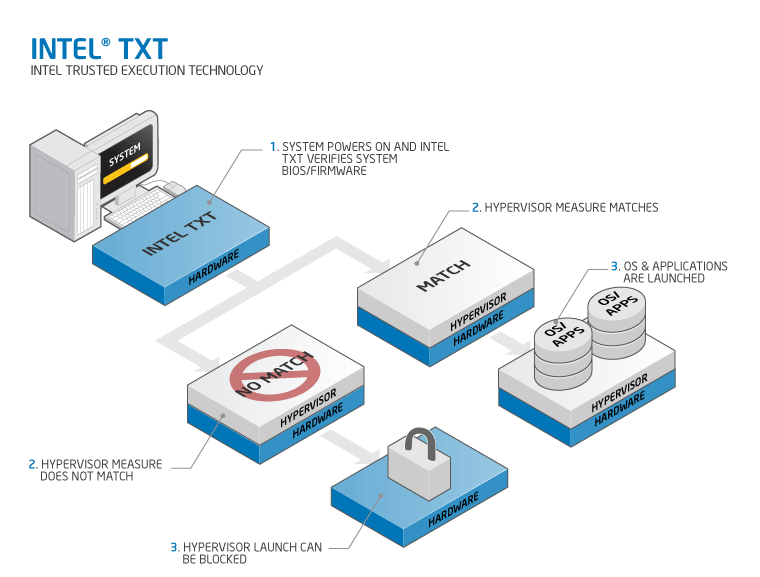
\includegraphics[scale=0.70]{attachements/techrefresh-info-txtfull.png}
% 	\caption{Intel Trusted Execution Technology}
% \end{figure}

\subsubsection{Sécurité multiniveau, multi catégorie (MLS ou MCS)}

Le modèle de sécurité multiniveau permet d'atteindre certains des buts fixés comme l'intégrité ou la confidentialité. Il repose sur la séparation des données en plusieurs domaines, imposant des règles limitant les intéractions de l'utilisateur.

\textbf{Bell-LaPaluda :} Ce modèle préserve la confidentialité de l'information en n'autorisant un sujet à écrire uniquement dans un niveau de confidentialité supérieur ou égal, et à ne lire que dans un niveau de sécurité inférieur ou égal. Ce modèle présente plusieurs inconvénients majeurs parce qu'il ne permet pas d'imposer des contraintes d'intégrité et ne permet pas de faire de disctinctions précise entre deux personnes possédant le même niveau d'accréditation.

\begin{figure}[h]
	\centering
	\includesvg{attachements/bell-lp}{0.45}
	\caption{Le modèle Bell-LaPadula}
\end{figure}

\textbf{Biba :} A contrario du modèle précédent, c'est l'intégrité qui est préservée, car seules les modifications dans un niveau de sécurité inférieur sont autorisée, et la lecture ne peut se faire que sur un niveau d'intégrité supérieur.

\begin{figure}[h]
	\centering
	\includesvg{attachements/biba}{0.45}
	\caption{Le modèle Biba}
\end{figure}

Ces deux modèles ne permettent pas d'atteindre plus d'un ou deux objectifs à la fois, et posent le problème de la sur-classification des données (toutes les données devenues confidentielles). Ceci conduit à l'introduction d'une méthode de déclassification, compromettant l'ensemble du modèle.

\subsubsection{Contrôle d'accès basé sur des rôles (RBAC)}

Plus qu'un modèle réel de contrôle, c'est un modèle d'administration permettant de simplifier le travail de l'administrateur d'un système utilisant un contrôle mandataire. Le principe du contrôle d'accès mandataire consiste à attribuer des rôles à chaque utilisateur de la machine. Ces rôles donnent ainsi accès à différents éléments du système. Par exemple, les rôles d'utilisateur, d'administrateur et de webmaster peuvent être définis et un utilisateur classique pourra se voir attribuer le rôle de webmaster lui autorisant de modifier les pages disponibles sur un serveur sans avoir besoin de donner un accès administrateur complet à cette personne.

\subsubsection{Application de règles de politiques securité par les types (Type Enforcement)}

Ce principe repose sur l'association d'un contexte de sécurité à chaque objets et processus. L'accès à un object par un processus doit correspondre à une règle de la politique de sécurité pour être autorisé. Ce modèle nécessite l'attribution d'un contexte de sécurité à tous les objets du système, y compris les fichiers présents sur les supports de stockage.

\subsection{Solutions disponibles}

Nous allons détailler les implémentations de ces modèles de sécurité dans certains systèmes d'exploitations, notamment les systèmes ``libres'', pour lesquels nous pouvons avoir accès au code source : Linux et la famille des BSD.

\subsubsection{SELinux}

SELinux est une implémentation d'un mécanisme de contrôle d'accès mandataire basé sur le ``type enforcement'', de niveau de sécurité/confidentialité non prédéfinis, et d'un contrôle d'accès basé sur les rôles. SELinux a été développé par la National Security Agency (NSA) et a été intégrée au noyau Linux une fois que l'architecture des Linux Security Modules fut mise en place. SELinux permet de contrôler à chaque appel système la validité de l'interaction par rapport aux définitions d'une politique. On associe à chaque objets et processus un context de sécurité. L'accès à un object par un processus doit correspondre à une règle de la politique SELinux pour être autorisé. Il faut noter que chaque décission est prise indépendamment des précédantes : SELinux n'as pas de mémoire des transitions effectuées sur un système. C'est cette limitation et la possibilité d'utiliser les flux d'informations indirects, donc non contrôlés par SELinux, qui ont poussé la création de PIGA.

\begin{list}{}{}
 \item \textbf{Contrainte pour l'administrateur :} Il faut décrire la totalité des intéractions possibles pour chaque programme présent sur un système. Il faut s'assurer du bon fonctionnement de ces politiques. Il n'existe pas d'outils pour valider les politiques SELinux. Seuls certains systèmes de fichiers supportent les attributs étendus nécessaires à la labelisation des fichiers présents sur les supports de stockage.
 \item \textbf{Avantages :} Séparation fine des privilèges et des rôles, intégrée dans le noyau. Des politiques ont déjà été écrites. Il existe une distribution facilitant le déploiement de ce type de protection : Fedora.
\end{list}

\subsubsection{PIGA}

L'ensemble désigné sous le nom de PIGA est le résultat de la thèse de Jérémy Briffaut ainsi que des contributions de l'équipe SDS du LIFO, et des étudiants de l'ENSIB. Il est constitué notement d'une surcouche à SELinux permettant de définir et imposer des propriétés de sécurité à l'echelle du système en plus des contrôles au niveau des intéractions effectués par SELinux. Il apporte une ``mémoire'' à SELinux. Un tel résultat est obtenu après génération du graphe complet des intéractions possibles et autorisées par une politique SELinux, recherche de chemins interdits, et consignation de ces chemins. Cette solution permet un contrôle plus avancé sur les flux d'information dans un système, qu'ils soient directs ou indirects.

\begin{list}{}{}
 \item \textbf{Contrainte pour l'administrateur :} Connaissance du langage de définition de propriété PIGA, maîtrise préalable de SELinux, prérequis matériels pour la ``compilation'' des politiques.
 \item \textbf{Avantages :} Un contrôle très fin sur les intéractions dans un système, restriction (statique) des privilèges maximale.
\end{list}

Le système d'exploitation PIGA-OS basé sur la recherche effectué sur PIGA a été vainqueur du concours Sec\&Si organisé par l'Agence Nationale pour la Recherche (ANR) \cite{PIGA}\cite{PIGA2}.

\subsubsection{grsecurity \& PaX}

\textsc{grsecurity} est une autre implémentation des mécanismes de contrôle d'accès mandataire et des listes de contrôle d'accès. Il permet aussi une gestion des droits basée sur les rôles. Souvent associé à \textsc{grsecurity}, PaX est un patch pour le noyau Linux ajoutant des restrictions et des contrôles sur les accès à la mémoire.

\begin{list}{}{}
 \item \textbf{Contrainte pour l'administrateur :} Certains programmes ne fonctionnent plus avec les restrictions implémentées par PaX.
 \item \textbf{Avantages :} Protection avancée de l'utilisation de la mémoire avec PaX (pile non exécutable, ...)
\end{list}

\subsection{TrustedBSD}

% TODO

\subsubsection{iptables}

iptables et un logiciel permettant de contrôler plus facilement netfilter, le parre-feu intégré au noyau Linux. Il permet entre autre de définir précisément quels ports et quelles intéractions avec le réseau sont autorisées sur une machine. Les règles iptables peuvent être modifiées dynamiquement pour autoriser ponctuellement une application à communiquer avec l'extérieur mais le comportement d'iptables est statique par défaut. iptables est un parre-feu à états, c'est à dire qu'il garde en mémoire les intéractions précédantes opur déterminer la légitimité des interactions suivantes.

\begin{list}{}{}
 \item \textbf{Contrainte pour l'administrateur :}
 \item \textbf{Avantages :}
\end{list}

\subsubsection{PIGA-SYSTRANS ou contextd}

contextd est un démon chargé de coordonner différents mécanismes de sécurité sur un système Linux. En effet, dans toutes les solutions décrites préédement, les programmes se voyaient attribués les droits dont ils avaient besoin pour toujours. Une application utilisant ponctuellement le réseau se voyait attribué le droit définitif d'utiliser un port.

\begin{list}{}{}
 \item \textbf{Contrainte pour l'administrateur :}
 \item \textbf{Avantages :}
\end{list}

% TODO & FIXME
% Pax = sécurité automatique
% SELinux, GrSec = MAC qui contrôle les accès directs
% PIGA = contrôle les accès indirects
% iptables contrôle le trafic réseau
% 
% contextd = chef d'orchestre + changement dynamique des règles des autres  mécanismes de protection pour adapter les permissions au domaine d'utilisation.
% 
% Chercher tous les systèmes de MAC/DAC/RBAC,...
% 
% Classer les MAC en fonction du travail à faire par l'administrateur ? en fonction d'où ils agissent ? par rapport à la logique interne (stateless ou statefull) ?


\newpage

\section{Déroulement du projet}

\subsection{Base utilisée pour le développement}

% \subsection{PIGA-OS, PIGA-SYSTRANS}

\subsubsection{SELinux, PIGA, contextd}

La solution retenue par Jérémy Briffaut et l'équipe SDS pour construire un système d'exploitation sécurisé est constituée de SELinux, PIGA, et de contextd. Ces trois éléments forment une suite de couche qui offrent progressivement un contrôle plus fin sur les interactions sur un système Linux, et permettent de garantir des propriétés fines et précises, mais en même temps générales.

\subsubsection{Gentoo Hardened}

Notre project ayant pour but potentiel, à terme, d'être intégré dans le système PIGA-OS, nous avons basé l'intégralité du développement sur la distribution Gentoo Hardened, qui propose une version du noyau modifiée. C'est donc à partir des noyaux Linux 2.6.32-r9 et r22 version hardened que nous avons travaillé.

\subsection{Systemtap}

\subsubsection{Principe de fonctionnement}

Nous avons ainsi commencé par utiliser Systemtap, un outil d'analyse du noyau grâce à des scripts qui ne nécessitent pas de modifier le code du noyau. Systemtap utilise les KProbes, et les Kretprobes\cite{IBMRBST} pour intervenir à différents endroits dans le déroulement des fonctions du noyau pour permettre à l'utilisateur de lire certaines variables ou de logger certains appels système. Le principe de fonctionnement de Systemtap est résumé par la Figure~\ref{IBMST}.

\begin{figure}[!ht]
	\centering
	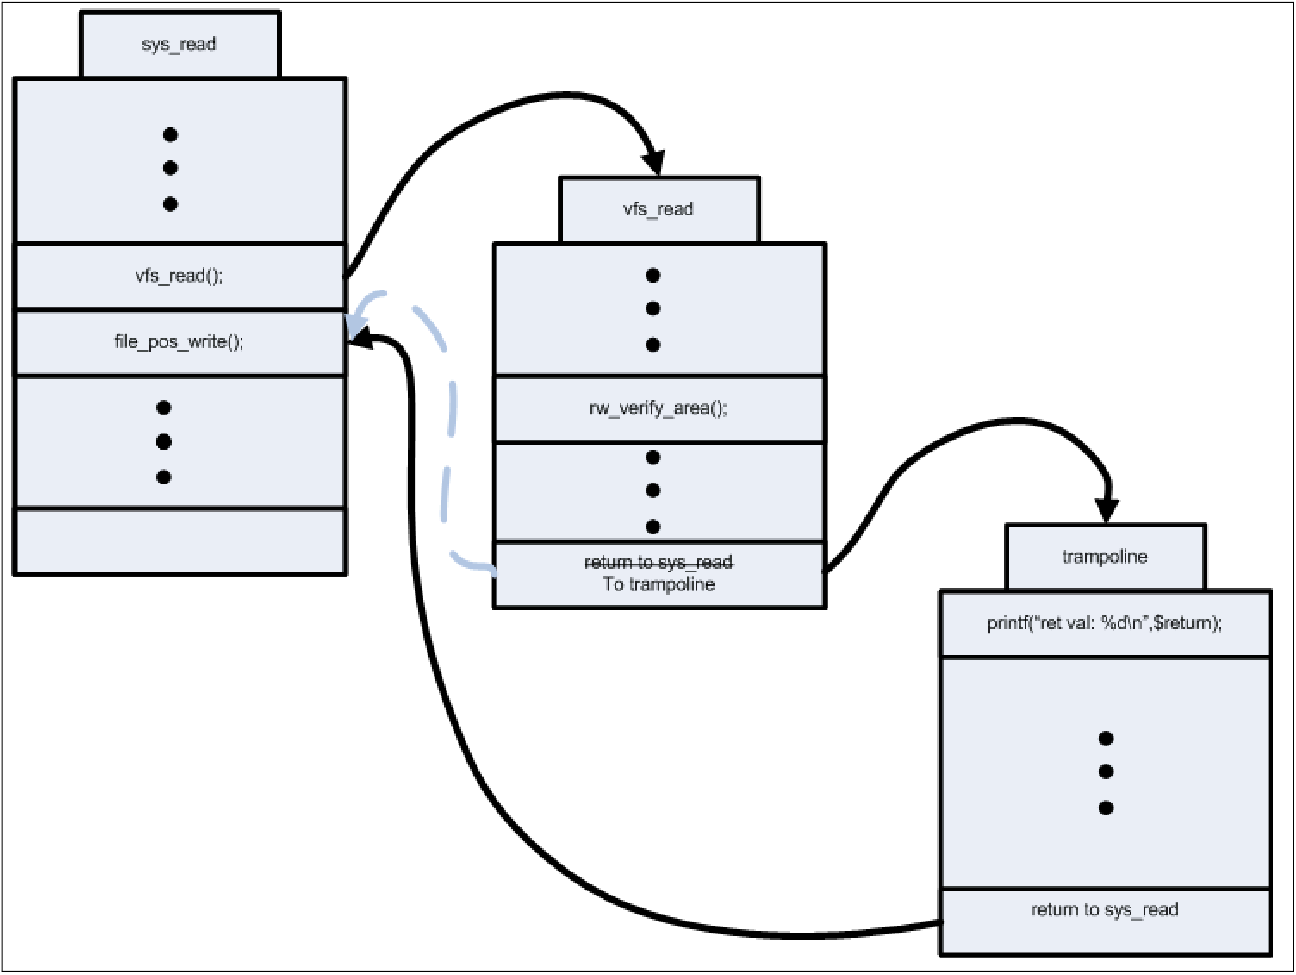
\includegraphics[scale=0.4]{attachements/kretprob.png}
	\caption{Fonctionnement tel que décrit dans la référence IBM sur Systemtap \cite{IBMRBST}}
	\label{IBMST}
\end{figure}

\subsubsection{Résultats obtenus}

Après s'être familiarisés avec le fonctionnement de Systemtap, nous nous sommes aperçu que les scripts utilisés pour récupérer les informations issues des appels système sont exécutés une fois l'appel système effectué. Il n'est pas possible, d'après nos recherches, de faire en sorte que les scripts puissent bloquer les appels système avant de les effectuer.

De ce fait, l'utilisation de Systemtap ne permet pas de répondre à nos besoins.

Il faut ajouter à cela que les informations recueillies à partir de Systemtap ne sont pas exploitables pour certaines d'entre-elles. Par exemple, lorsqu'un fichier est accédé (lu ou écrit), seul le numéro d'inode nous était retourné. Il n'était alors pas pertinent de récupérer le chemin complet du fichier, car cette recherche est inadaptée et inefficace : il est nécessaire de parcourir l'intégralité du système de fichiers.

Il fallait donc changer de stratégie. C'est pourquoi, nous avons, avec l'accord du responsable du projet, décidé de nous orienter vers l'utilisation des ``Linux Security Modules'' (LSM).

\section{Solution retenue et implémentée}

La solution retenue est axée sur les modules LSM.

\subsection{Linux Security Modules}

Les modules LSM sont au noyau ce que netfilter est au réseau.

Le principe de fonctionnement est simple : un module LSM est chargé dans le noyau Linux au démarrage. Il se substitue ou complète alors la procédure de contrôle d'accès. \`A chaque appel système est associé un point d'ancrage ou hook que l'on peut considérer comme une fonction. Il est placé dans l'appel système entre les vérifications élémentaires (existence des fichiers, droits unix) et sa réalisation. Dès qu'un appel système est demandé, le hook est exécuté. Par défaut, il autorise l'exécution de l'appel système.

\begin{figure}[!ht]
	\centering
	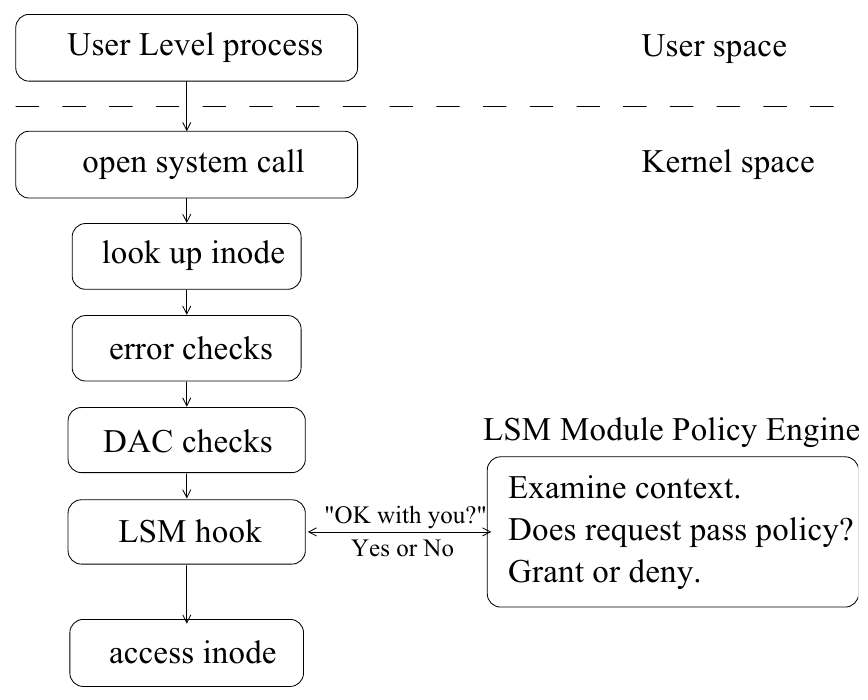
\includegraphics[scale=0.45]{attachements/lsm1.png}
	\caption{Architecture des hooks LSM \cite{LSMINTRO}}
\end{figure}

L'avantage de ces hooks est qu'ils offrent une très grande liberté. Cependant, il n'est possible pour le moment de ne charger dans le noyau qu'un seul et unique module LSM. Or, PIGA-OS utilise déjà un module LSM : SELinux.

\begin{figure}[!ht]
	\centering
	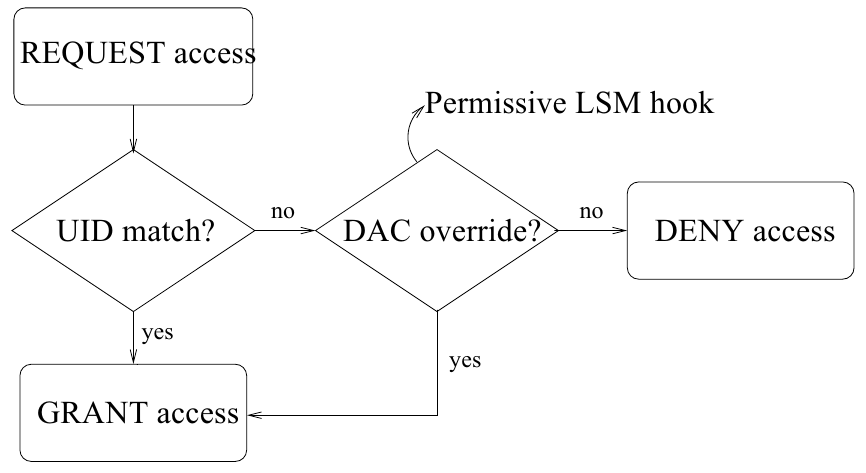
\includegraphics[scale=0.45]{attachements/lsm2.png}
	\caption{Hook LSM permissif. Ce hook autorise la politique de sécurité à passer outre les restrictions DAC \cite{LSMINTRO}}
\end{figure}

Pour les besoins du développement, nous avons dû désactiver SELinux, pour nous concentrer sur notre propre module, et non sur l'intégration avec le module LSM de SELinux.

\subsection{Détail de la solution}

Nous avons donc décider de nous orienter vers l'implémentation d'un module LSM. Grâce aux "hooks", et notamment la fonction "file\_permission", nous pouvons contrôler les différents accès aux ressources systèmes telles que les fichiers (binaires ou textes).

Nous avons également remarqué que les hooks ``socket\_bind'' et ``socket\_connect'' permettent de récupérer des informations, notamment l'adresse IP et le port de destination d'une socket, avant qu'elle ne soit créée. Il existe également deux autres "hooks" ``socket\_recvmsg'' et ``socket\_sendmsg'' qui permettent, eux, de pouvoir exercer un contrôle en fonction du contenu du paquet. On peut donc imaginer grâce à ces quatre "hooks" pouvoir surveiller les connexions réseaux.

Par manque de temps, nous avons décidé de ne pas surveiller ces "hooks". Cependant, nous avons tout mis en œuvre afin que les informations disponibles dans ces "hook" arrivent à contextd, afin, de pouvoir travailler sur l'exploitation des données et effectuer les contrôles voulus à l'avenir.

En effet, contextd ne permet pas de prendre de décisions sur les adresses IP mais seulement sur les URLs. Une requête DNS inverse ne permet malheureusement pas d'obtenir d'adresse utilisable par contextd. Nous n'avons donc pas poursuivi l'intégration des ``connexions'' dans notre solution.

La principale difficulté de cette étape fut de localiser dans quels fichiers ces informations sont définies parmi l'ensemble du code source du noyau Linux. S'agissant de structures pour la plupart, il nous fallait savoir quels en étaient les membres pour pouvoir en tirer les informations essentielles au fonctionnement de contextd.

Nous avons donc dû étudier également le fonctionnement du démon contextd. Il s'avère qu'il n'a besoin que de peu de données et se contente de :
	\begin{itemize}
		\item le PID
		\item l'execname
		\item le chemin complet du fichier
		\item le context de sécurité SELinux~\\
	\end{itemize}
	
\textit{\textsl{\textbf{Nota bene :}}} Pour les activités réseaux, contextd à besoin de non seulement du FQDN mais aussi de la page et/ou des sous-domaines associés. Bien qu'il puisse utiliser des adresses IP, ce comportement n'est pas souhaitable pour des raisons évidentes liées au fonctionnement d'Internet. En revanche, le noyau n'a conscience que de l'adresse IP associée à une connexion. Il faut donc pouvoir retrouver à partir de l'IP le FQDN. Après une tentative, grâce à la fonction \textit{getnamebyaddr}, nous n'avons pas pu retrouver un FQDN exploitable. En effet, nous avons tenté une connexion vers www.google.fr afin de voir, si à partir de l'adresse IP résolue, nous pouvions retrouver google. Force est de constater que le résultat, wy-in-f104.1e100.net, bien qu'il redirige vers google, n'est pas exploitable par contextd.

Maintenant que ces informations sont localisées, il faut pouvoir les extraire de l'espace noyau (kernel space) pour les acheminer dans l'espace utilisateur (userspace) là où opère contextd.

\subsection{Problématique de la communication entre contextd et le noyau}

Compte tenu du fonctionnement de contextd, il a fallu développer un système de communication entre le noyau et contextd.

\begin{figure}[!ht]
	\centering
	\includesvg{attachements/contextd_dbus}{0.45}
	\caption{Communication entre contextd et les applications}
	\label{contextd_dbus}
\end{figure}

En effet, comme le montre la Figure~\ref{contextd_dbus}, l'implémentation choisie au départ pour acheminer les informations nécessaires à contextd était centrée sur DBus, un système de communication inter-processus simple.

\subsubsection{Les appels systèmes}

Pour mettre en place la communication entre l'espace noyau et le démon en espace utilisateur contextd, nous avons implémenté trois nouveaux appels système. En effet, la solution des appels système nous permet de contrôler les interactions avec le noyau en créant :
\begin{itemize}
 \item \textbf{auditsec\_reg} : démarre/termine la communication et enregistre/désinscrit les programmes à surveiller.
 \item \textbf{auditsec\_question} : bloquant, qui attend une demande d'autorisation de la part du noyau.
 \item \textbf{auditsec\_answer} : qui permet de donner une réponse au noyau.\\
\end{itemize}

\begin{figure}[!ht]
	\centering
	\includepic{attachements/sequence_diagram}{1}
	\caption{Diagramme de séquence entre le noyau, contextd, et une application}
\end{figure}

Nous utilisons des mutex pour s'assurer du traitement par contextd de chacun des appels système.

\begin{figure}[!ht]
	\centering
	\includesvg{attachements/syscall_sync}{0.6}
	\caption{Communication entre les hooks LSM et les appels système}
\end{figure}

Une fois que contextd est enregistré, toute nouvelle tentative d'enregistrement échouera. Il sera nécessaire de quitter contextd avant d'effectuer un nouvel enregistrement. Cela permet de limiter la communication par l'intermédiaire de cet appel, pour l'enregistrement et la désinscription des programmes à surveiller.

Les appels système présentent deux avantages majeurs par rapport à d'autres solutions :
\begin{itemize}
  \item l'appel auditsec\_question est bloquant, laissant le processus en attente d'une réponse du noyau. Cela évite d'avoir à vérifier périodiquement l'état d'un fichier contenant temporairement des informations.
  \item il n'est pas nécessaire de parser les informations reçues : nous utilisons un pointeur sur une structure remplie par le noyau.\\
\end{itemize}

En revanche, il est peu probable qu'une telle solution soit acceptée par les développeurs du noyau. Il faudrait donc envisager de convertir ces appels systèmes en appels à ioctl, un appel système utilisé pour communiquer avec les périphériques par exemple.

\subsubsection{L'interface présentée à l'administrateur}

Pour simplifier la tâche de l'administrateur et rendre compte de l'état du noyau, nous avons créé les ``proc files''. Ce système de fichiers virtuel, contenu dans la mémoire vive du système, permet non seulement de récupérer des informations depuis le noyau mais aussi de lui en envoyer.

Nous avons mis en place deux fichiers dans l'arborescence /proc :

	\begin{itemize}
		\item \textbf{/proc/contextd/programs} : Ce fichier liste les programmes qui ont été enregistrés auprès du noyau et qui sont donc surveillés. Des demandes seront envoyées à contextd pour ces programmes. Ce fichier n'est disponible qu'en lecture seule. En effet, nous considérons qu'une fois contextd lancé, lui seul peut décider de l'enregistrement ou de la désincription d'un programme.
		\item \textbf{/proc/contextd/status} : Ce fichier est en revanche accessible en lecture et en écriture. En lecture, on y trouve le pid de contextd (plus précisément le tgid, pour ne pas prendre en compte les threads de contextd). En écriture, s'il reçoit un 0, le noyau désactive la surveillance par contextd et vide la liste des programmes enregistrés. Il est donc impératif que ce fichier ne soit pas accessible par défaut à un utilisateur non privilégié. On peut aussi envisager de désactiver ce comportement sur un système en production.
	\end{itemize}

\subsubsection{Séparation des fonctions de communications dans contextd}

Nous avons dû modifier contextd afin de lui ajouter la possibilité de communiquer avec le noyau grâce aux appels système que nous avions définis. Pour ce faire, nous nous sommes inspiré de ce qui était déjà implémenté, à savoir la communication par l'intermédiaire de DBus.

Cette communication se faisait grâce à la classe "DBusContext". Cette classe traitait les sollicitations des clients (programmes), les enregistrait dans une table de hashage privée et s'occupait des transitions. Les programmes étaient indexés par le dbus\_id correspondant au canal de communication DBus.

Nous avons donc reproduit ce comportement pour la réception des informations depuis le noyau. Nous avons créé une classe "KernelContext" qui permet de traiter le cas des processus non modifiés et ne disposant pas de plugin.

Pour éviter une potentielle surveillance double, nous avons décidé d'abstraire le comportement de ces deux classes recevant de l'information à transmettre à contextd. Nous avons donc pallié ce problème en implémentant une classe abstraite "AbstractContext" afin de centraliser la liste des clients pour toutes les sources d'information. Les classes DBusContext et KernelContext héritent alors de la classe AbstractContext qui possède la liste des clients en attribut static protégé : ces propriétés permettent à toutes les classes qui héritent d'AbstractContext d'avoir accès à l'instanciation de cette liste sans que celle-ci ne dépende d'une instance en particulier. L'accès à la liste des clients est synchronisé pour éviter toute concurrence d'accès.

Dans le cas où un troisième mode de communication serait envisagé, il sera alors aisé de faire les modifications pour que celui-ci s'intègre parfaitement à ce qui existe déjà : il suffira d'hériter de la classe AbstractContext.

\begin{figure}[!ht]
	\centering
	\includedot{attachements/class}{.8}
	\caption{Diagramme de classes}
\end{figure}

\subsubsection{Surveillance et enregistrement dynamique}

Pour rendre contextd conscient de nos modifications nous avons implémenté plusieurs éléments :

\begin{itemize}
	\item L'enregistrement et la désinscription/mise à jour de la liste des programmes surveillés par contextd lors de la réception du signal SIGUSR2.
	\item La vérification de la cohérence de la liste des clients stockée par contextd : cette liste est maintenant nettoyée à intervalles réguliers.
\end{itemize}

De plus, notre solution nécessitant maintenant l'enregistrement des programmes auprès du noyau, il est désormais possible de charger dynamique cette liste de programmes à partir de /etc/context.d/program.d. Il est par contre nécessaire de préciser à contextd, à la compilation, les programmes à exclure de cette liste (pour l'instant firefox, claws-mail et context-notify).

\textit{\textsl{\textbf{Nota bene :}}} Nous partons du principe que notre travail est/sera utilisé avec SELinux, même si ce n'est pas possible actuellement. Nous n'effectuons aucune vérification d'intégrité sur les programmes surveillés par contextd. Cette intégrité est en principe assurée par les politiques SELinux et/ou les règles PIGA.

\section{Implémentation}

\subsection{Ajout du module dans le menuconfig et la compilation du noyau}

Premièrement, nous avons donc développé un module LSM qui "hook" les appels système. Pour ce faire, nous avons créé un dossier "auditsec" dans \textit{{kernel\_src}/security/}. C'est dans ce dossier que nous avons mis toutes nos sources (appels système, hook, etc.) ainsi qu'un sous dossier \textit{{kernel\_src}/security/includes} pour nos headers.

Ensuite,  pour avoir la possibilité d'activer ou non ce module lors de la compilation du noyau (suivant les conventions de nommage des options de configuration) il a fallu ajouter la ligne suivante dans \textit{{kernel\_src}/security/Kconfig} :


\begin{lstlisting}[language=make]
source security/auditsec/Kconfig
\end{lstlisting}

Il faut ajouter également un fichier Kconfig dans le dossier \textit{{kernel\_src}/security/auditsec} pour définir la description, le type de variable et le texte du menuconfig. Dans ce fichier, on insère les lignes suivantes :

\begin{lstlisting}[language=make]
config SECURITY_AUDITSEC
bool "Userspace contextd capture LSM hook"
depends on AUDIT && NET && INET
select NETWORK_SECMARK
default n
help
 Module pour communiquer avec contextd pour la gestion d'applications en userspace.
\end{lstlisting}

La description des différentes lignes ci-dessus :
\begin{itemize}
	\item Nom de la variable. On pourra l'utiliser avec des "\#ifdef" dans le code C. La variable sera alors "CONFIG\_SECURITY\_AUDITSEC".
	\item Type de variable pour menuconfig (ici booléen)
	\item De quel autre partie de configuration notre module a besoin.
	\item Active d'autres options
	\item Par défaut, le module est désactivé.
	\item La description
\end{itemize}

 Pour que ce dossier soit pris en compte lors de la compilation, il faut rajouter les lignes suivantes dans \textit{{kernel\_src}/security/Makefile} :

\begin{lstlisting}[language=make]
subdir-$(CONFIG_SECURITY_AUDITSEC)  += auditsec	
obj-$(CONFIG_SECURITY_AUDITSEC)     += auditsec/built-in.o
\end{lstlisting}

Puis, il faut ajouter un Makefile dans notre dossier \textit{{kernel\_src}/security/auditsec/Makefile} :

\begin{lstlisting}[language=make]
obj-$(CONFIG_SECURITY_AUDITSEC) := audit_security.o
 
audit_security-y := hooks.o share.o syscall.o

EXTRA_CFLAGS += -Isecurity/auditsec/include
$\end{lstlisting}

Ceci fait, tout est désormais prêt pour la compilation. Maintenant, passons à la création d'un module LSM. L'implémentation de ce module a été faite dans le fichier \textit{{kernel\_src}/security/auditsec/hook.c}. 

\subsection{Création des éléments nécessaires au module}

La particularité d'un module LSM est l'utilisation d'une structure spéciale qui liste les différentes fonctions appelées lorsqu'un appel système est demandé. Voici donc la structure de notre module.

\begin{lstlisting}[language=C]
static struct security_operations audit_ops = {
	.name =             "audit_ops", // nom 
	.inode_mkdir =                  auditsec_inode_mkdir,
	.file_permission =              auditsec_file_permission,
	.socket_bind =                  auditsec_socket_bind,
	.socket_connect =               auditsec_socket_connect,
	.socket_sendmsg =               auditsec_socket_sendmsg,
 	.socket_recvmsg =               auditsec_socket_recvmsg
 };
\end{lstlisting}

Il faut donc ajouter le code de ces six hooks. Pour connaître la signature de ces fonctions, il faut aller voir dans \textit{{kernel\_src}/security/security.c}. 

Par exemple, voici le code de la fonction auditsec\_file\_permission:

\begin{lstlisting}[language=C]
int auditsec_file_permission(struct file *file, int mask)
{
...
	if(prog_is_monitored()){ // On teste si le programme est surveille
...
		// On recupere le chemin complet du fichier auquel on accede
		file_path(file, fullpath);
		if(*daemon_launched()){  // On teste si contextd est lance
			if(down_timeout(auditsec_hook_lock(), 30 * HZ) != 0){...}
			
			// On remplit la structure
			get_task_comm(k_auditsec_info()->execname, current);
			k_auditsec_info()->pid = current_pid;
			k_auditsec_info()->type = AUDITSEC_FILE;
			strncpy(k_auditsec_info()->auditsec_struct.file.fullpath, fullpath, PATH_MAX + 1);
			strncpy(k_auditsec_info()->auditsec_struct.file.name, file->f_path.dentry->d_name.name, NAME_MAX + 1);
			k_auditsec_info()->auditsec_struct.file.mask = mask;
			
			// La structure est prete, on leve le verrou pour que contextd puisse la recuperer
			up(auditsec_question_lock());
			
			// On attend la reponse
			if(down_timeout(auditsec_answer_lock(), 30 * HZ) != 0){...}
			
			// On a eu la reponse			
			answer = (*auditsec_answer() == 0);
			up(auditsec_hook_lock());

			// On autorise ou non suivant la reponse (0 oui - -EACCES non)
			return answer == 0 ? 0 : -EACCES;
		}else{...}
	}else{...}
	return 0;
}
\end{lstlisting}

\subsubsection{Liste des programmes surveillés}

Comme on peut le voir, le code de ce "hook" fait appel à plusieurs éléments. Tout d'abord, on teste si le programme qui a déclenché ce "hook" est surveillé par contextd. Pour ce faire, on a crée une liste au niveau du noyau contenant l'ensemble des programmes surveillés par contextd. On traitera plus tard de la manière dont cette liste est mise à jour.

Nous définissons une structure pour stocker un programme :

\textit{{kernel\_src}/security/auditsec/include/share.h} :
\begin{lstlisting}{language=C}
struct prog {
	char execname[TASK_COMM_LEN];
	struct list_head list;
};
\end{lstlisting}

Puis nous déclarons la liste des programmes en utilisant une des implémentation de liste générique du noyau :

\textit{{kernel\_src}/security/auditsec/share.c} :
\begin{lstlisting}[language=C]
static LIST_HEAD(prog_list);
\end{lstlisting} 

Maintenant, pour tester si une application appartient à cette liste, nous faisons appel à la fonction suivante :

\textit{{kernel\_src}/security/auditsec/share.c} :
\begin{lstlisting} [language=C]
int prog_is_monitored()
{
	char current_task_comm[TASK_COMM_LEN];
	struct prog * p;

	get_task_comm(current_task_comm, current);
	list_for_each_entry(p, &prog_list, list){
		if(strncmp(p->execname, current_task_comm, TASK_COMM_LEN) == 0){
			printk(KERN_INFO "AuditSec: Prog %s is monitored", current_task_comm);
			return 1;
		}
	}
	return 0;
}
\end{lstlisting} 

Enfin, il faut pouvoir ajouter ou supprimer des éléments de cette liste. Nous avons implémenté pour cela les fonctions suivantes :

\textit{{kernel\_src}/security/auditsec/share.c} :
\begin{lstlisting} [language=C]
int register_prog(char * prog_name)
{
	struct prog * p;

	printk(KERN_INFO "AuditSec: Registering prog %s", prog_name);
	list_for_each_entry(p, &prog_list, list) {
		if(strncmp(p->execname, prog_name, TASK_COMM_LEN) == 0){
			printk(KERN_INFO "AuditSec: Prog %s already registered", prog_name);
			return -1;
		}
	}

	p = kmalloc(sizeof(*p), GFP_NOFS);
	if(p == NULL){
		return -ENOMEM;
	}
	strncpy(p->execname, prog_name, TASK_COMM_LEN);
	INIT_LIST_HEAD(&p->list);

	list_add(&p->list, &prog_list);
	printk(KERN_INFO "AuditSec: Prog %s registered", prog_name);
	return 0;
}


int unregister_prog(char * prog_name)
{
	struct prog * p;

	if(list_empty(&prog_list) != 0){
		printk(KERN_INFO "AuditSec: Prog list empty !");
		return -1;
	}

	list_for_each_entry(p, &prog_list, list) {
		if(strncmp(p->execname, prog_name, TASK_COMM_LEN) == 0){
			list_del(&p->list);
			kfree(p);
			printk(KERN_INFO "AuditSec: Unregistering prog %s", prog_name);
			return 0;
		}
	}

	return -1;
}
\end{lstlisting} 

\subsubsection{Structure transmise}

Une fois les tests effectués, le "hook" remplie une structure. Nous avons opté pour une structure "dynamique" plutôt qu'une multitude de structure car les données sont différentes selon le "hook" surveillé.

La partie principale de cette structure est la suivante :

\textit{{kernel\_src}/security/auditsec/struct.c} :
\begin{lstlisting} [language=C]
enum auditsec_type {AUDITSEC_FILE, AUDITSEC_SOCKET, AUDITSEC_DIR, AUDITSEC_MSG};

struct auditsec_info {
    pid_t       pid;
    char        execname[TASK_COMM_LEN];
    //FIXME Add SELinux context to this struct
    enum        auditsec_type type;
    union
    {  
        struct auditsec_file file;
        struct auditsec_socket socket;
        struct auditsec_dir dir;
        struct auditsec_msg msg;
    } auditsec_struct;
};
\end{lstlisting} 

Ainsi seule "auditsec\_struct" variera suivant les "hooks" qui la rempliront. Nous avons donc créé différentes structures pour chaque type de "hook".

Concernant les fichiers :

\textit{{kernel\_src}/security/auditsec/struct.c} :
\begin{lstlisting} [language=C]
struct auditsec_file {
    char        name[NAME_MAX + 1];
    char        fullpath[PATH_MAX + 1];
    int         mask;
};
\end{lstlisting} 

Concernant les dossiers : 

\textit{{kernel\_src}/security/auditsec/struct.c} :
\begin{lstlisting} [language=C]
struct auditsec_dir {
    char        name[NAME_MAX + 1];
    char        fullpath[PATH_MAX + 1];
    int         mode;
};
\end{lstlisting} 

Concernant les sockets : 

\textit{{kernel\_src}/security/auditsec/struct.c} :
\begin{lstlisting} [language=C]
enum socket_type {AUDITSEC_IPV4, AUDITSEC_IPV6};

struct auditsec_socket {
    enum        socket_type type;
    union
    {
        struct sockaddr_in  addr4; // Adresse ip V4
        struct sockaddr_in6  addr6; // Adresse ip V6
    } addr;
};

struct auditsec_msg {
    struct msghdr msg;
    int size;
};
\end{lstlisting} 

\subsubsection{Création du module}

Maintenant que tous les éléments nécessaires sont définis, il faut maintenant implémenter la fonction d'initialisation du module. Lors de cette initialisation, doivent être créés les "proc files" ainsi que les fonctions nécessaires pour les lire et/ou écrire dedans.

\textit{{kernel\_src}/security/auditsec/hooks.c} :
\begin{lstlisting} [language=C]
static __init int auditsec_init(void)
{
	struct proc_dir_entry * auditsec_proc_programs, *auditsec_proc_status, *auditsec_dir;

	if (!security_module_enable(&audit_ops)) {
		printk(KERN_INFO "AuditSec: Abort initialization.\n");
		return 0;
	}

	printk(KERN_INFO "AuditSec: Initializing.\n");

	if (register_security(&audit_ops))
		panic("AuditSec: Unable to register with kernel.\n");

	init_MUTEX(auditsec_hook_lock());
	init_MUTEX(auditsec_question_lock());
	init_MUTEX(auditsec_answer_lock());

	down(auditsec_question_lock());
	down(auditsec_answer_lock());

	// Create dir in /proc
	auditsec_dir = proc_mkdir(PROC_AUDITSEC_DIR, NULL);

	if (auditsec_dir == NULL) {
		printk(KERN_INFO "AuditSec: failed to creat /proc/%s/ directory", PROC_AUDITSEC_DIR);
		return -ENOMEM;
	}

	// Create file in /proc/PROC_AUDITSEC_DIR/ which lists registered programs
	auditsec_proc_programs = create_proc_entry(PROC_AUDITSEC_PROGRAM, 0400, auditsec_dir);

	if (auditsec_proc_programs == NULL) {
		printk(KERN_INFO "AuditSec: failed to creat /proc/%s/%s file", PROC_AUDITSEC_DIR, PROC_AUDITSEC_PROGRAM);
		remove_proc_entry(PROC_AUDITSEC_PROGRAM, auditsec_dir);
		return -ENOMEM;
	}

	auditsec_proc_programs->read_proc    = auditsec_proc_programs_read;
	auditsec_proc_programs->mode         = S_IFREG | S_IRUGO;
	auditsec_proc_programs->uid          = 0;
	auditsec_proc_programs->gid          = 0;
	auditsec_proc_programs->size         = 0;

	// Create file in /proc/PROC_AUDITSEC_DIR/ which gives the current status and
	// the opportunity to change it
	auditsec_proc_status = create_proc_entry(PROC_AUDITSEC_STATUS, 0600, auditsec_dir);

	if (auditsec_proc_programs == NULL) {
		printk(KERN_INFO "AuditSec: failed to creat /proc/%s/%s file", PROC_AUDITSEC_DIR, PROC_AUDITSEC_STATUS);
		remove_proc_entry(PROC_AUDITSEC_STATUS, auditsec_dir);
		return -ENOMEM;
	}

	auditsec_proc_status->read_proc    = auditsec_proc_status_read;
	auditsec_proc_status->write_proc   = auditsec_proc_status_write;
	auditsec_proc_status->mode         = S_IFREG | S_IRUGO;
	auditsec_proc_status->uid          = 0;
	auditsec_proc_status->gid          = 0;
	auditsec_proc_status->size         = 0;

	printk(KERN_INFO "AuditSec: Waiting for daemon.\n");

	return 0;
}

security_initcall(auditsec_init);
\end{lstlisting}

\subsubsection{Fonctions de lecture pour \textit{/proc/contextd/programs}}

L'initialisation du module et la création des proc files nécessitent l'implémentation également des fonctions qui permettront la lecture et l'écriture dans ces fichiers. Pour pouvoir lire le fichier \textit{/proc/contextd/programs}, nous avons implémenté la fonction suivante :

\textit{{kernel\_src}/security/auditsec/hooks.c} :
\begin{lstlisting} [language=C]
int auditsec_proc_programs_read(char *buffer, char **buffer_location,  off_t offset, int buffer_length, int *eof, void *data)
{
	int result = 0;
	char * tmp = NULL;
	
	if (offset > 0) {
		/* we have finished to read, return 0 */
		result  = 0;
	} else {
		/* fill the buffer, return the buffer size */
		tmp = prog_liste();
		result = sprintf(buffer, "%s", tmp);
		kfree(tmp);
	}

	return result;
}
\end{lstlisting}

\subsubsection{Fonctions de lecture/écriture pour \textit{/proc/contextd/status}}

Concernant ce proc file, il faut deux fonctions car il est accessible en lecture et écriture. En lecture il fournit le pid qu'il considère comme être celui de contextd ; en écriture, il permet, si on envoie "0" de désactiver la surveillance et de vider la liste des programmes surveillés.

\textit{{kernel\_src}/security/auditsec/hooks.c} :
\begin{lstlisting} [language=C]
int auditsec_proc_status_read(char *buffer, char **buffer_location,  off_t offset, int buffer_length, int *eof, void *data)
{
	int result;
	
	if (offset > 0) {
		/* we have finished to read, return 0 */
		result  = 0;
	} else {
		/* fill the buffer, return the buffer size */
		result = sprintf(buffer, "%d\n", *contextd_pid());
	}

	return result;
}

int auditsec_proc_status_write(struct file *file, const char *buffer, unsigned long count, void *data)
{
	long lecture;
	char tmp[count + 1];
	char ** tmp2 = NULL;

	if(copy_from_user(tmp, buffer, count)){ 
		return -EFAULT;
	}

	tmp[count] = '\0';

	lecture = simple_strtol(tmp, tmp2, 10);

	if (lecture == 0){
		*daemon_launched() = false;
		*contextd_pid() = -1;
		clean_prog_list();
	}

	return 0;
}
\end{lstlisting}

Voici donc le module LSM complet et fonctionnel. Nous avons vu comment étaient implémentées les différentes composantes dont il a besoin pour fonctionner. Au tour des appels système.

\subsection{Les appels système}

\subsubsection{ausitsec\_reg}

Cet appel système a une quadruple fonction :
\begin{itemize}
	\item Enregistrer contextd auprès du noyau.
	\item Ajouter les programmes surveillés.
	\item Dé-enregistrer des programmes pour ne plus les surveiller.
	\item Dé-enregistrer contextd.
\end{itemize}

Il s'assure aussi de l'identité de l'appelant, ne laissant qu'à contextd, une fois lancé, la possibilité de modifier la liste des programmes à surveiller. Voici le code source de cet appel système :

\textit{{kernel\_src}/security/auditsec/syscall.c} :
\begin{lstlisting} [language=C]
asmlinkage long sys_auditsec_reg(int __user state, char __user * process_name)
{
	// Contextd isn't registered yet
	if(*contextd_pid() == -1){
		if(state == 1){
			if(process_name == NULL){
				*contextd_pid() = task_tgid_nr(current);
				*daemon_launched() = true;
				printk(KERN_INFO "AuditSec: The daemon is now considered launched");
				return 1;
			}else{
				printk(KERN_INFO "AuditSec: The daemon is not launched: can't register a program !");
				return 0;
			}
		}else if(state == 0){
			printk(KERN_INFO "AuditSec: According to the kernel, the daemon is already stopped");
			return 0;
		}else{
			printk(KERN_INFO "AuditSec: Invalid state provided !");
			return 0;
		}

	// Contextd is already registered
	}else if(*contextd_pid() == task_tgid_nr(current)){
		if(state == 1){
			if(process_name == NULL){
				printk(KERN_INFO "AuditSec: According to the kernel, the daemon is already launched");
				return 1;
			}else{
				printk(KERN_INFO "AuditSec: Registering program: %s", process_name);
				if(register_prog(process_name) == 0){
					printk(KERN_INFO "AuditSec: Program registered: %s", process_name);
					return 1;
				}else{
					printk(KERN_INFO "AuditSec: Program NOT registered: %s", process_name);
					return -1;
				}
			}
		}else if(state == 0){
			if(process_name == NULL){
				*contextd_pid() = -1;
				*daemon_launched() = false;
				clean_prog_list();
				printk(KERN_INFO "AuditSec: The daemon is now considered stopped. Program list emptied");
				return 0;
			}else{
				printk(KERN_INFO "AuditSec: Unregistering program: %s", process_name);
				if(unregister_prog(process_name) == 0){
					printk(KERN_INFO "AuditSec: Program unregistered: %s", process_name);
					return 1;
				}else{
					printk(KERN_INFO "AuditSec: Error: Program: %s", process_name);
					return -1;
				}
			}
		}

	// Contextd is registered but access is denied to other process
	}else{
		printk(KERN_INFO "AuditSec: You're not contextd");
	}
	printk(KERN_INFO "AuditSec: No action performed");
	return -EFAULT;
}
\end{lstlisting}

\subsubsection{ausitsec\_question}

Cet appel système attend, grâce aux jeux des verrous que la structure de données soit remplie par le "hook".

\textit{{kernel\_src}/security/auditsec/syscall.c} :
\begin{lstlisting} [language=C]
asmlinkage long sys_auditsec_question(struct auditsec_info __user * user_as_i)
{
	if(*daemon_launched() == false){...}

	if(*contextd_pid() != task_tgid_nr(current)){...}

	if(down_interruptible(auditsec_question_lock()) != 0){...}

	if(likely(user_as_i != NULL)){
		if(likely(copy_to_user(user_as_i, k_auditsec_info(), sizeof(struct auditsec_info)) == 0)){
			return 0;
		}
	}
	// If an error occured during the copy, the transaction is rejected
	*auditsec_answer() = false;
	up(auditsec_answer_lock());
	printk(KERN_INFO "AuditSec: Process %d, error in data transfer to userspace.", task_pid_nr(current));

	return -EFAULT;
}
\end{lstlisting}

Pour partager les verrous entre les appels système et les ``hooks'', nous avons défini les fonctions :

\textit{{kernel\_src}/security/auditsec/share.c} :
\begin{lstlisting} [language=C]
struct semaphore * auditsec_hook_lock()
{
	static DECLARE_MUTEX(auditsec_hook_lock);
	return &auditsec_hook_lock;
}

struct semaphore * auditsec_question_lock(){...}

struct semaphore * auditsec_answer_lock(){...}
\end{lstlisting}

\subsubsection{auditsec\_answer}

Cet appel système transmet la réponse de contextd au noyau. Voici son implémentation :
\textit{{kernel\_src}/security/auditsec/syscall.c} :
\begin{lstlisting} [language=C]
asmlinkage long sys_auditsec_answer(int __user answer)
{
	if(*daemon_launched() == false){...}

	if(*contextd_pid() != task_tgid_nr(current)){...}

	*auditsec_answer() = answer;
	up(auditsec_answer_lock());

	return 0;
}
\end{lstlisting}

\subsubsection{Déclaration des appels système}

Une dernière étape est cependant nécessaire pour que ces appels système soient pleinement opérationnels. Il faut les déclarer. Pour cela, nous avons ajouté les lignes suivantes dans le fichier \textit{{kernel\_src}/include/linux/syscalls.h} :

\begin{lstlisting} [language=C]
asmlinkage long sys_auditsec_reg(int __user state, char __user *);
asmlinkage long sys_auditsec_question(struct auditsec_info __user *);
asmlinkage long sys_auditsec_answer(int __user);
\end{lstlisting}

Ensuite, il faut attribuer aux appels système un numéro. Cela est fait en ajoutant les lignes suivantes dans le fichier \textit{{kernel\_src}/arch/x86/kernel/syscall\_table\_32.S} : %en notant les numéros !

\begin{lstlisting}[language=C]
	.long sys_auditsec_reg
	.long sys_auditsec_question
	.long sys_auditsec_answer
\end{lstlisting}

et enfin :

\textit{{kernel\_src}/arch/x86/include/asm/unistd\_64.h}
\begin{lstlisting}[language=C]
#define __NR_auditsec_reg			299
__SYSCALL(__NR_auditsec_reg, sys_auditsec_reg)
#define __NR_auditsec_question			300
__SYSCALL(__NR_auditsec_question, sys_auditsec_question)
#define __NR_auditsec_answer			301
__SYSCALL(__NR_auditsec_answer, sys_auditsec_answer)
\end{lstlisting}

Grâce à tout ce qui précède, nous sommes en mesure de stopper les appels systèmes des applications surveillées, de communiquer avec le noyau et de récupérer les informations essentielles pour pouvoir prendre une décision sur l'accès ou non à la ressource demandée.

\subsection{Modification de contextd}

Maintenant, voyons les modifications apportées à contextd. Comme cela a été dit précédemment, la principale modification apportée à contextd concerne le mode de communication avec les applications. Initialement, une seule classe existait pour gérer la communication qui ne se faisait que via DBus.

\subsubsection{Ajout d'une classe ``AbstractContext''}

Nous nous sommes inspiré de la classe ``DBusContext'' pour créer la classe abstraire. Nous n'avons implémenté qu'une seule et unique méthode \textit{getFullPathFromPID} qui sera, quoi qu'il advienne, toujours la même y compris pour les classes dérivées.

De plus, pour partager la liste de clients (les applications surveillées et enregistrées), nous avons déclaré cette liste en tant qu'attribut de cette classe abstraite. Voici le code produit :

\textit{abstractcontext.h} : 
\begin{lstlisting}[language=C++]
class AbstractContext : public QObject
{
Q_OBJECT
protected:
	//There is some concurrency here. Use the lock!
	static QMap<pid_t, ContextClient> clients;
	static QReadWriteLock lock;

	QString getFullPathFromPID(pid_t pid);

public slots:
	virtual QString register_application(const QString &app_name, uint app_pid) = 0;

	virtual QString domain_changed(const QString &xml_context) = 0;
	virtual QString required_domain(const QString &xml_context) = 0;

	virtual QString current_domain() = 0;
	virtual QString is_registered() = 0;

	virtual QString register_for_domain_changes_updates() = 0;

protected slots:
	virtual void onGlobalContextChanged(Domain previousGlobalContext, Domain globalContext) = 0;

	void onEvent(ContextdPluginEvent* event);

signals:
	void globalContextChanged(const QString &previous_context, const QString &new_context);
};
\end{lstlisting}

\textit{abstractcontext.cpp} : 
\begin{lstlisting}[language=C++]
QMap< pid_t, ContextClient > AbstractContext::clients;

QReadWriteLock AbstractContext::lock;


QString AbstractContext::getFullPathFromPID(pid_t pid)
{
	QString proc_path="/proc/%1/exe";
	proc_path=proc_path.arg(pid);

	return QFile::readLink(proc_path);
}


void AbstractContext::onEvent(ContextdPluginEvent* event)
{
	if(event->type()==ContextdPluginRestartEvent().type())
	{
		DomainHolder::instance().resetToDefaultDomain();
	}
}
\end{lstlisting}

\subsubsection{Modification de ``DBusContext''}

Compte tenu que la précédente liste de client était indexée par le dbus\_id, et que les programmes dont l'enregistrement se fait via le noyau ne dispose pas d'un tel identifiant, il a fallut modifier les méthodes de cette case. La modification est très succincte : il a juste fallu ajouter ces quelques lignes dans les méthodes et de modifier dbus\_id en pid.

\textit{dbus-context.cpp} : 
\begin{lstlisting}[language=C++]
	//Get the pid
	QDBusReply<uint> res = QDBusConnection::systemBus().interface()->servicePid(dbus_id);
	if(res.isValid()){
		pid = res.value();
	}else{
		return DBUS_ERROR;
	}
\end{lstlisting}

\subsubsection{Ajout de la classe ``KernelContext''}

Enfin, nous avons implémenté la classe KernelContext qui hérite d'AbstractContext. Elle utilise un QThread (KThread) pour gérer la boucle de communication avec le noyau.

\textit{auditsec\_lsm/kthread.h} :
\begin{lstlisting}[language=C++]
class KThread : public QThread
{
Q_OBJECT
public:
	KThread(KernelContext *);
	void run();

	bool _keep_going;

private:
	KernelContext * KC;
	QString xmlContext(char *, ...);
	QString toXMLEntities(QString str);
};
\end{lstlisting}

\textit{auditsec\_lsm/kthread.cpp} :
\begin{lstlisting}[language=C++]
KThread::KThread(KernelContext * kc) : KC(kc)
{
	_keep_going = true;
}


void KThread::run()
{
	QString address;
	struct sockaddr_in addr_;
	struct hostent * hote = NULL;

	while(_keep_going && (auditsec_question(KC->usai()) == 0)){
		if(KC->is_registered() == KERNEL_ERROR){
			KC->register_application(KC->usai()->execname);
		}

		switch (KC->usai()->type){
			case AUDITSEC_FILE:
				qDebug() << "KThread: File: " << KC->usai()->auditsec_struct.file.fullpath;
				KC->domain_changed(xmlContext(
					"fullpath", KC->usai()->auditsec_struct.file.fullpath,
					//"filename", KC->usai()->auditsec_struct.file.name,
					NULL, NULL));
				break;

			case AUDITSEC_DIR:
				...
				break;
			
			case AUDITSEC_SOCKET:
				...
				break;

			default:
				...
				break;
		}
	}
}
\end{lstlisting}

\section{Résultats finaux}

La Figure~\ref{SCHEMAFIN} résume le fonctionnement de contextd avec toutes les modifications que nous avons apportées.

\begin{figure}[!ht]
	\centering
	\includesvg{attachements/fonctionnement_apres}{1.3}
	\caption{Schéma de fonctionnement}
	\label{SCHEMAFIN}
\end{figure}

\subsection{Avec un programme de test}

Les tests que nous avons conduit nous amènent à penser que notre travail correspond globalement à ce qui était attendu. En effet, le programme de test "testprog" montre que le comportement du système est cohérent avec les règles contextd écrites. Le programme testprog se contente d'afficher le contenu de fichiers placés dans des répertoires aux noms explicites :

\begin{lstlisting}[language=C++]
int openfile(std::string filename){...}

int main(int argc, char ** argv)
{
	for (int i=0; i < 2; i++) {
		openfile("/home/user/impots/test");
		openfile("/home/user/ecommerce/test");
	}
	return 0;
}
\end{lstlisting}

Les Figures~\ref{INI}, \ref{DEMANDE} et \ref{FIN} détaillent ce test, qui présente un cas d'utilisation de contextd.

Tout d'abord, sur la Figure~\ref{INI}, nous lançons contextd qui va essayer de s'enregistrer auprès du noyau, puis va charger les plugins internes contenant les fonctionnalités de contextd. Il se place alors en attente d'événements. Le premier qu'il a à traiter correspond à l'enregistrement de context-notify à travers DBus (terminal en haut à gauche). Le lancement de context-notify est affiché dans le terminal en haut à droite. Enfin, nous affichons les messages envoyés par le noyau avec la commande dmesg : seuls les quatre derniers correspondent à cette instance de contextd et indiquent l'enregistrement de firefox, soffice.bin et testprog (terminal en bas à droite). Les messages précédents correspondent à ceux envoyés lors de l'extinction de contextd.

\begin{figure}[h]
	\centering
	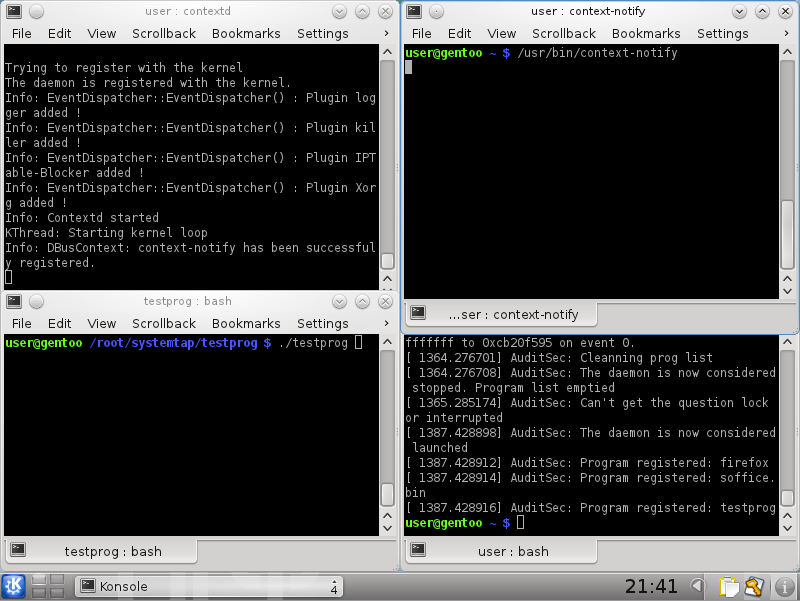
\includegraphics[scale=0.5]{attachements/capture_ini.png}
	\caption{Après lancement de contextd}
	\label{INI}
\end{figure}

La Figure~\ref{DEMANDE} correspond à l'affichage lorsque ce programme de test tente d'ouvrir un fichier qui appartient à un autre domaine que le domaine actuel (ici default). Si la transaction est autorisée par les règles établies pour testprog et qu'il est précisé que l'utilisateur doit confirmer cette action, une demande est envoyée à context-notify qui attend la réponse pour la renvoyer à contextd. Si l'utilisateur met trop de temps à répondre (30 secondes actuellement), la demande est rejetée et il ne se produit aucun changement de domaine.

\begin{figure}%[!ht]
	\centering
	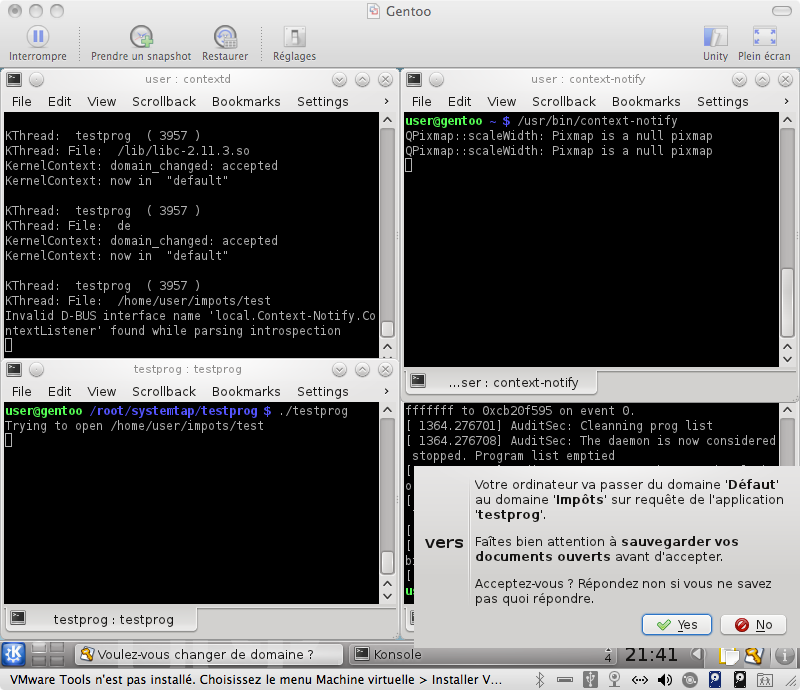
\includegraphics[scale=0.5]{attachements/capture_notify.png}
	\caption{Après lancement de progtest}
	\label{DEMANDE}
\end{figure}

\begin{figure}
	\centering
	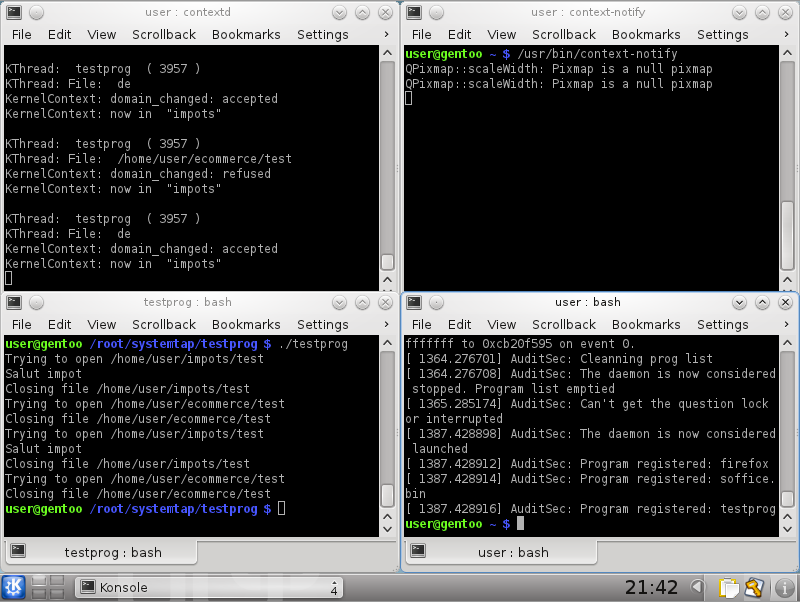
\includegraphics[scale=0.5]{attachements/capture_fin.png}
	\caption{Après confirmation du changement de domaine}
	\label{FIN}
\end{figure}

La Figure~\ref{FIN} présente le résultat final. Dans ce cas de figure, il n'y a eu qu'une seule demande de changement de domaine car nous avons configuré contextd de telle sorte que les domaines soient des puits (cf les fichiers de configurations associés aux programmes dans /etc/context.d/program.d/mon\_programme.xml et le fichier décrivant les transitions autorisées /etc/context.d/transitions.xml). Ainsi, une fois dans le domaine ``impôts'', testprog peut afficher les données du dossier impôts mais pas celles du dossier ecommerce. L'affichage dans le terminal en haut à gauche détaille les demandes de transitions et les réponses de contextd.

D'autres tests effectués avec Libreoffice, montrent que le résultat fonctionne parfaitement avec des programmes classiques et courants sans aucune modification. Cependant, les erreurs affichées par ces applications ne sont pas forcément très explicites (Libreoffice considère parfois que le document est endommagé alors que le noyau lui a refusé l'accès). Ce problème est lié au choix de LSM : les applications ne peuvent pas faire la différence entre un refus lié aux permissions classiques et un refus lié au module de sécurité. Ces mêmes cas de figure se produisent sur un système utilisant SELinux, lors des refus de transitions de contexte.

Pour finir, voici un extrait du fichier de configuration pour testprog :

\begin{lstlisting}[language=XML]
		<!-- Loop -->
		<loop app_name="testprog" notify="false" prompt="false" display_name="Loop">
			<matching>
				<mrule>
					<fullpath>(/usr/lib/.*|/lib/.*|de|s|/etc/resolv.conf|/etc/nsswitch.conf|/etc/host.conf|/etc/hosts)</fullpath>
				</mrule>
			</matching>
			<domains>
				<loop_domain name="default" />
				<loop_domain name="mail" />
				<loop_domain name="web" />
				<loop_domain name="web-flash" />
				<loop_domain name="ecommerce" />
				<loop_domain name="impots" />
			</domains>
		</loop>

		<!--Impots-->
		<rule app_name="testprog" to_domain="impots" notify="false" prompt="true" display_name="domaine impots">
			<matching>
				<mrule>
					<fullpath>(/home/user/impots/.*)</fullpath>
				</mrule>
			</matching>
			<transitions>
				<allow>
					<transit from_domain="impots" notify="false" prompt="false"/>
					<!--<transit from_domain="ecommerce" to_domain="impots" notify="false" prompt="true"/>-->
					<transit from_domain="default" />
				</allow>
			</transitions>
		</rule>

		<!--Ecommerce-->
		<rule app_name="testprog" to_domain="ecommerce" notify="false" prompt="true" display_name="domaine ecommerce">
			<matching>
				<mrule>
					<fullpath>(/home/user/ecommerce/.*)</fullpath>
				</mrule>
			</matching>
			<transitions>
				<allow>
					<transit from_domain="ecommerce" notify="false" prompt="false"/>
					<!--<transit from_domain="mail" to_domain="ecommerce" prompt="true" />-->
					<transit from_domain="default" to_domain="ecommerce" prompt="true" />
					<!--<transit from_domain="impots" to_domain="ecommerce" prompt="true" />-->
				</allow>
			</transitions>
		</rule>
\end{lstlisting}

\subsection{Poursuite du projet}

Les éléments suivant restent à réaliser avant d'envisager l'intégration de notre travail dans PIGA-OS :
	\begin{itemize}
		\item Les règles à fournir à contextd pour définir les accès autorisés pour un programme deviennent rapidement compliquées car elles doivent être exhaustives (il faut notamment autoriser le chargement de toutes les librairies pour les programmes non compilés en statique, ...). L'usage des expressions régulières réduit cet impact mais ne résout pas le prblème.
		\item Nous avons pris pour base un module LSM vide. Il faut en revanche intégrer nos modifications au module SELinux pour pouvoir faire fonctionner notre solution avec PIGA-OS. Il faudrait aussi envisager la solution des empilements de modules LSM et s'assurer de l'usage de notre module.
		\item Enfin, il faut noter qu'il n'est pour l'instant pas possible de se séparer complètement des plugins, en particulier pour les applications devant modifier leur comportement interne lors d'un changement de domaine (claws-mail, firefox). Notre solution permet juste de réduire le travail de ``portage'' d'une application vers PIGA-SYSTRANS.
	\end{itemize}

\newpage

% \section{Résultats et benchmarks}
% 
% Benchmark : Sans le module LSM, Avec le module mais pas lancé, Avec le module et lancé
% 
% \newpage

\section*{Conclusion} \addcontentsline{toc}{section}{Conclusion}

Le but de ce projet était de simplifier l'ajout d'application à PIGA-SYSTRANS et au système PIGA-OS. Cet objectif est atteint car nos travaux permettent, par exemple, de faire fonctionner OpenOffice.org/LibreOffice avec contextd, sans modifier ces applications.

De plus, l'aspect totalement générique de notre solution nous assure un fort potentiel de réutilisation. En effet, les ajouts dans contextd permettant le chargement dynamique de programmes à contrôler nous permettent de se concentrer sur l'écriture de règles contextd, et non sur la modification des applications.

Il ne reste alors plus qu'à modifier uniquement les applications possédant un comportement s'étendant sur plusieurs domaines et dont l'état interne nécessite des modifications lors d'un changement de domaine. Pour l'instant, les applications concernées sont Mozilla Firefox et Claws-Mail. Il est difficilement envisageable de se ``débarrasser'' du plugin Claws-Mail à l'avenir. Mais l'arrivée de la séparation entre les onglets sous Firefox et du principe un onglet = un processus pourrait permettre de se séparer du plugin Firefox.

Enfin, il faut noter que notre projet ne prendra tout son sens que lorsqu'il sera intégrable à PIGA-OS. Ce n'est pour l'instant pas le cas, mais les modifications restantes restent moindres par rapport aux objectifs atteints par ce projet. Un essai d'intégration à été réalisé, mais aucun test ni vérification de fonctionnalité n'a été effectué par manque de temps.

Nous tenons à remercier Jérémy Briffaut et Martin Peres pour leur aide précieuse tout au long du déroulement de ce projet.

% Le retard, sur la partie implémentation noyau, par rapport à notre planification est principalement dû à notre découverte très progressive des capacités offertes aux développeurs. Le livre Linux Kernel Development \cite{LKDTE} nous a permis de faire un bon en avant dans la compréhension du fonctionnement du noyau et notamment l'implémentation des appels système.

\newpage
% \addcontentsline{toc}{section}{Annexes}
\addcontentsline{toc}{section}{Références}

% \subsection*{Liens et références}
\begin{thebibliography}{40}

\bibitem{IBMRBST} Bart Jacob, Paul Larson, Breno Henrique Leitao, Saulo Augusto M Martins da Silva, \textit{IBM Redbooks : SystemTap: Instrumenting the Linux Kernel for Analyzing Performance and Functional Problems}, \url{http://www.redbooks.ibm.com/abstracts/redp4469.html}

\bibitem{LSMINTRO} Chris Wright, Crispin Cowan, Stephen Smalley, James Morris, Greg Kroah-Hartman, \textit{Linux Security Modules : General Security Support for the Linux Kernel}, \url{http://citeseerx.ist.psu.edu/viewdoc/download?doi=10.1.1.84.6867&rep=rep1&type=pdf}

\bibitem{LKDSE} Robert Love, \textit{Linux Kernel Development, Second Edition}, Novell Press
\bibitem{LKDTE} Robert Love, \textit{Linux Kernel Development, Third Edition}, Pearson Education, Inc.

\bibitem{SELEX} Frank Mayer, Karl MacMillan, David Caplan, \textit{SELinux By Example}, Prentice Hall, Première édition, 6 août 2006
\bibitem{MRHEL5} Daniel J Walsh, Karl MacMillan, \textit{Managing Red Hat Enterprise Linux 5}, \url{http://people.redhat.com/dwalsh/SELinux/Presentations/ManageRHEL5.pdf}

\bibitem{WCS} \textit{Wikipedia : Computer Security}, \url{http://en.wikipedia.org/wiki/Computer_security}

\bibitem{SOURCE} Code source (kernel 2.6.32 hardened r22, piga-systrans, et scripts systemtap) disponible sur le serveur de projet STI (le projet s'appelle Contextd Capture), \url{http://projetsti.ensi-bourges.fr/projects/promo2012-systemtap}.

\bibitem{TIOF} Peter A. Loscocco, Stephen D. Smalley, Patrick A. Muckelbauer, Ruth C. Taylor, S. Jeff Turner, and John F. Farrell. The Inevitability of Failure : The Flawed Assumption of Security in Modern Computing Environments. In Proceedings of the 21st National Information Systems Security Conference, pages 303–314, Arlington, Virginia, USA, October 1998

\bibitem{QNX} QNX Realtime Operating System, \url{http://www.qnx.com}

\bibitem{ITXT} Intel Trusted Execution Technology (TXT), \url{http://www.intel.com/technology/malwarereduction/index.htm}

\bibitem{PIGA} Jérémy Briffaut, Martin Peres, Jonathan Rouzaud-Cornabas, Jigar Solanki, Christian Toinard, Benjamin Venelle, \textit{PIGA-OS : Retour sur le système d'exploitation vainqueur du défi sécurité}

\bibitem{PIGA2} Jérémy Briffaut, Jean-François Lalande, Christian Toinard, \textit{Formalization os security properties : enforcement for mac operating systems and verification of dynamic mac policies}, International journal on advances in security, 2:325-343, 2009

\end{thebibliography}

%\printindex

\end{document}
